\documentclass[11pt,a4paper,twoside]{book}
\usepackage[utf8]{inputenc}
\usepackage[spanish]{babel}
\usepackage{amsmath}
\usepackage{graphicx}
\usepackage{amsfonts}
\usepackage{amssymb}
\usepackage[left=2cm,right=2cm,top=2cm,bottom=2cm]{geometry}
\author{Víctor de Tejada Molera}
\begin{document}
    \chapter{Realización de los tests subjetivos de audio}
        \section{Test preliminar}
            En primer lugar se plantea la realización de un pequeño test subjetivo de audio cuyo objetivo es la comprobación rápida de que la hipótesis de partida es correcta. Esta hipótesis es que los oyentes perciben de forma distinta el sonido en función de la distancia de la que se encuentren de una fuente sonora y que dicha percepción es suficientemente similar para posiciones simétricas dentro del espacio de estudio. Es decir, que las dimensiones y características de la sala permitan que la distancia sea un factor perceptible por los oyentes y que el salón de actos sea lo suficientemente simétrico para poder simplificar la toma de respuestas al impulso.
            
            \subsection{Características del test previo}
                Para la realziación de este test, se ha optado por seguir las recomendaciones propuestas en (REFERENCIAVDT). Para ello, el proyecto propone responder a las siguientes preguntas:
                \begin{itemize}
                    \item \textbf{¿En qué categoría se engloba el estudio?}: Para responder a esta pregunta, hay que observar las diferentes categorías que se presentan en el artículo (Inteligibilidad, Sensibilidad, Reverberación, Localización y Molestia). Para el caso de este test, el que más se corresponde es el de Sensibilidad, puesto que el objetivo es ver si las personas participantes tienen la capacidad para distinguir si los sonidos son iguales o no.
                    \item \textbf{¿Qué tipo de test es el más adecuado?}: Para los objetivos de este test, se ha optado por un test 2-AFC también conocido como \textit{Same/Different}. Este tipo de test obliga al participante a elegir entre dos opciones; en nuestro caso, si los audios que se presentan son iguales o diferentes. Esto tiene la ventaja de que es fácil de codificar y analizar estadísticamente aunque no da mucha información concreta, pero es suficiente para el objetivo del test.
                    \item \textbf{¿Participantes expertos o inexpertos?,¿cuántos necesito?}: Como este test no es el definitivo, sino que se trata de una comprobación previa, no se han considerado requisitos tan estrictos como los que se hubieran seguido de otra forma. Por este motivo, se ha optado por utilizar participantes con y sin experiencia. El número total de participantes ha sido de 10 que es lo mínimo que se ha utilizado en algunos test de temática similar (REFERENCIA10PARTICIPANTES).
                    \item \textbf{¿Qué tipo de señal utilizo?}: En nuestro caso, se utilizan las respuestas al impulso convolucionadas obtenidas previamente del salón de actos siguiendo el procedimiento seguido en el capítulo de "Toma de datos". En concreto para este experimento se han utilizado las respuestas de las zonas más cercanas y lejanas a la fuente en las posiciones centrales y de los extremos laterales tanto izquierdo como derecho.
                    \item \textbf{¿Cuál es tipo de análisis de datos?}: Para el análisis de los datos, se ha optado por realizar un análisis del coeficiente $\alpha$ de acuerdo con las especificaciones de la norma ISO-10399 (REFERENCIAISO). En dicha norma, se proporciona una tabla que muestra el número de respuestas correctas necesarias para concluir que dos eventos son diferentes con una determinada incertidumbre para un determinado número de respuestas totales.
                \end{itemize}
                
                La escucha de los diferentes audios y la inclusión de las respuestas se realiza mediante una interfaz gráfica diseñada en el lenguaje de programación Python utilizando la librería de código abierto GTK. En el apartado ``Desarrollo de aplicación en Python''. En la figura \ref{fig:interfazInicial} se puede observar la interfaz utilizada en el test previo.
                
                \begin{figure}
                    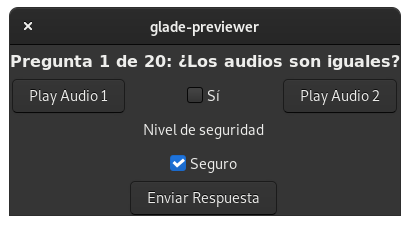
\includegraphics[scale=0.6]{../imagenes/uiIni.png}
			        \centering
			        \caption{Interfaz gráfica para la realización del test previo.}
			        \label{fig:interfazInicial}
                \end{figure}
            \subsection{Procedimiento del test previo}
                Una vez determinadas todas las características del test previo, se empieza a realizar el test de forma individual a cada uno de los diez participantes. La sala donde se realizaron las escuchas fue una de las salas de laboratorio del Centro de Investigación en Tecnologías Software y Sistemas Multimedia para la Sostenibilidad (CITSEM). Esta sala se encuentra aislada de las zonas de tránsito y sus ventanas no dan a zonas con tráfico. De esta forma, se pueden controlar fácilmente las fuentes de ruido ajenas al experimento. Es importante remarcar que, debido a la pandemia producidad por la COVID-19, las ventanas tienen que estar abiertas en todo momento con el fin de conseguir unas condiciones de ventilación apropiadas que evitaran posibles contagios. Este es el motivo por el que se optara por una sala que cuyas ventanas no dieran a fuentes de ruido externas.
                
                El equipo utilizado consistió en un ordenador portátil con sistema operativo Debian con 12GB de memoria RAM y unos auriculares Tascam-TH02. Previa a las escuchas por parte de los participantes, se aseguró de que las señales se reprodujeran con un nivel adecuado. Al principio del test, se les explicaba a los participantes las carácterísticas del test que iban a relizar, así como el número de preguntas y en qué propiedades debían fijarse para facilitarles su realización. Una vez finalizada la realización del test y ,debido al carácter no definitivo del mismo, se les preguntó sobre posibles mejoras que se podían hacer para facilitar su realización como cambios en la interfaz gráfica, la inclusión de audios de ejemplo, etc. 
            
        \section{Características de los tests finales}
            Como ya se comentó en el apartado del análisis del estado del arte, no existe un consenso sobre la mejor forma de realizar un test subjetivo de audio. Algunos estudios como REFERENCIAVICTOR y REFERENCIADELAPRIDA hacen algunas sugerencias sobre qué características pueden funcionar mejor en función de lo que se pretenda analizar en dicho test. Para nuestro caso particular, se ha vuelto a optar por seguir las recomendaciones propuestas en REFERENCIAVICTOR respondiendo a las preguntas que en él se plantean. Como ya se comentó en el apartado de ``Toma de datos'', se tuvieron que repetir los test de audio debido a un fallo en el procesado de las grabaciones. A pesar de esto, las características de ambas pruebas son prácticamente idénticas. Por este motivo, se engloban las características de ambos en el mismo apartado. Dentro de cada subapartado se comentan, si existen, las diferencias que pueda haber entre ambos.
            
            \begin{itemize}
                
                \item \textbf{¿En qué categoría se engloba el estudo?}: Al igual que en el test previo, se pretende determinar la sensibilidad que tienen las personas para distinguir las diferencias perceptuales al escuchar sonidos cuando se encuentran en distintas posiciones respecto de la fuente acústica. Por este motivo, se puede concluir que este test se encuentra englobado dentro de los que se consideran como de Sensibilidad.
                \item \textbf{¿Qué tipo de test es el más adecuado?}: Para el estudio que se pretende hacer, existen numerosos tipos de test que pueden arrojar datos interesantes. Entre ellos, los dos más habituales son los de referencia oculta como ABX o los Duo-Trio. No obstante, se ha optado por repetir el tipo de test utilizado en el estudio previo; es decir 2-AFC o \textit{Same-Different}. Los motivos que han llevado a esta elección han sido la facilidad de implementación y codificación, su simpleza que lo hace apropiado para todo tipo de participantes y que permite arrojar resultados bastante fiables mediante un análisis relativamente sencillo usando modelos Thurstonianos, además de que existen normas internacionales que permiten obtener resultado extra que pueden ser interesantes de comparar con los de los modelos.
                \item \textbf{¿Participantes expertos o inexpertos?, ¿cuántos necesito?}: A la hora de plantear el experimento, desde un primer momento se planteó como una situación que afectaba a la población general. Por este motivo, se consideró que no era especialmente relevante que los participantes tuvieran una especial experiencia en la realización de este tipo de test, aunque obviamente, es necesario que no padezcan de ninguna afección auditiva que afecte a su nivel de audición, ya sea por la edad, enfermedad, etc. A pesar de todo esto, se consideró que todas personas participantes debían pasar por una breve sesión de entrenamiento previo para que supieran de antemano en qué elementos de los sonidos tenían que fijarse. Estas indicaciones vienen reflejadas en las normas REFERENCIASNORMAS que muestran la utilidad de este tipo de entrenamientos para obtener mejores resultados.
                
                En cuanto al número de participantes totales, se siguieron las recomendaciones de las mismas normas, así como las conclusiones extraídas de REFERENCIAVICTOR y de los otros experimentos consultados de temática similar REFERENCIASENSIBILIDAD. De esta forma, se concluyó que el número de participantes debían de ser de un mínimo de 30 personas.
                \item \textbf{¿Qué tipo de señal utilizo?}: Las señales utilizadas para la realización del primer test fueron los archivos de audio generados tras la convolución de la voz femenina obtenida en REFERENCIAVOZ con cada una de las respuestas impulsivas grabadas en el salón de actos de la ETSIST de la UPM. El proceso de la obtención de dichas respuestas se encuentra explicado en el apartado de ``Toma de datos''. Se trata de un total de 100 archivos de audio de 7 segundos de duración. Esta duración se encuentra dentro de los límites marcados por REFERENCIANORMAS para evitar que los oyentes se ``acostumbre'' al  sonido. Así mismo, se encuentra dentro del abánico de duraciones que se ha observado en distintos proyectos de similares características. \newline
                
                Para el segundo test, se optó por utilizar diréctamente las respuestas al impulso obtenidas tras el procesado que realiza el software \textit{Dirac}, como ya se explica también en el apartado de ``Toma de datos''. En este caso, se utilizan un total de 83 archivos distintos de 2 segundos de duración. Al igual que en la prueba anterior, la duración se encuentra dentro de los límites marcados por REFERENCIANORMAS y otros estudios para evitar la fatiga auditiva y que los participantes se acostumbren a los estímulos.
                
                Para la realización de ambos experimentos, el volumen al cual se reproducen las señales no es relevante, siempre y cuando no se modifique a lo largo de toda la sesión; por lo que el participante puede escoger el que le fuera más cómodo, con la única restricción de que el volumen debe ser el mismo para la escucha de los dos audios que conforman cada pregunta.
                \item \textbf{¿Cuál es el tipo de análisis de datos?}
            \end{itemize}
        \section{Procedimiento del test}
        
            \subsection*{Localización}
                En primer lugar, se organizaron los turnos para la realización del test. El espacio escogido para la realización de las escuchas consistió en un laboratorio del CITSEM localizado en el Campus Sur de la UPM. Se escogió esta localización porque, debido a la situación pandémica producida por el COVID-19, era necesario que las ventanas estuvieran abiertas en todo momento. Se planteó la utilización de aparatos de depuración del aire, pero su ruido era comparable o más molesto todavía que la realización del mismo con las ventanas abiertas. No obstante, se escogió una localización donde las ventanas daban a una zona poco transitada, tanto por peatones como por vehículos, de forma que se conseguía un ambiente suficientemente controlado y silencioso. Si antes de comenzar el test se consideraba que el ruido externo era mayor del habitual, se cerraban las ventanas durante su realización y se volvían a abrir al finalizar el experimento.
            
            \subsection*{Material utilizado}
                Para la realización de ambos test se utilizó el mismo material que en el test preliminar. En concreto:
                \begin{itemize}
                    \item Ordenador portátil con S.O. Debian 11 con procesador \textit{intel} i5 y 12GB de RAM.
                    \item Auriculares Tascam-TH02.
                    \item declaraciones de consentimiento.
                    \item software \textit{Gnome Builder} para la ejecución de la aplicación.
                \end{itemize}
                
            \subsection*{Realización del test}
                En primer lugar, todas las personas participantes debían inscribirse en un cronograma con el fin de poder organizar las entradas y salidas evitando que se produjeran acumulaciones de personas en espacios cerrados. Una vez inscritas y cuando llegaba su turno, se les explicaba brevemente en qué consistía el experimento del que iban a formar parte y se les daba a leer una hoja de información al participante en el que se explica en mayor detalle las particularidades del test, las partes de la que consta, así como información relevante en temas de salud y protección de datos. Una vez leído, debían rellenar una declaración responsable aceptando los aspectos marcados en el documento anterior. Ambos documentos pueden consultarse en su totalidad en el Anexo X.
                
                A continuación daba comienzo el test con el tutorial. En él se le presenta al participante tres de las posibilidades que podría encontrarse (que los audios fueran de la misma posición, que fueran de filas distintas y que fueran de butacas distintas de la misma fila). Como el objetivo de este tutorial es que sepan identificar qué aspectos determinan que audios sean iguales o diferentes, para los tres casos se optó por utilizar casos críticos, estos son aquellos que se utilizaban las mismas posiciones que en el test previo, donde las posiciones eran lo más separadas posibles. La reproducción de los audios se podía repetir el número de veces que se considerara necesario. En la figura \ref{fig:interfazTutorial} puede observarse la interfaz de dicha parte.
                
                \begin{figure}
                    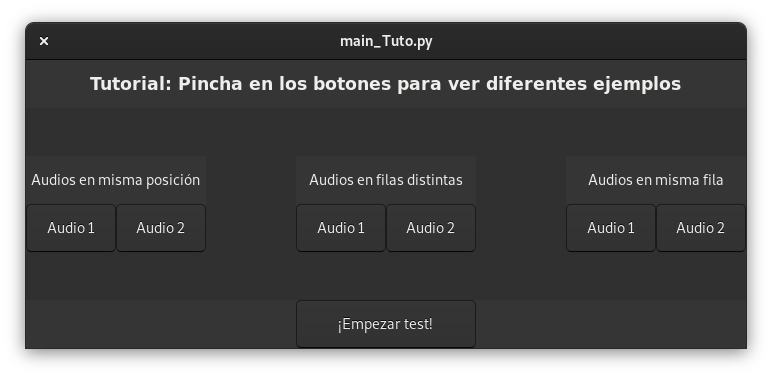
\includegraphics[scale=0.6]{../imagenes/interfaz_tutorial.png}
			        \centering
			        \caption{Aapriencia del entrenamiento previo}
			        \label{fig:interfazTutorial}
                \end{figure}
                
                Una vez el participante consideraba que estaba preparado, pulsaba el botón de ``Comenzar el test'' para dar inicio a la segunda parte.
                
                En esta segunda parte al usuario se le presentan dos audios convolucionados de forma aleatoria y debe determinar si lo que percibe son dos audios que suenan igual o no. Por otro lado, el participante debe especificar si se encuentra seguro de su respuesta. El usuario puede repetir la reproducción de los audios las veces que quiera, pero debe esperar a que el audio termine de reproducirse antes de poder escoger si repetirlo o escuchar el otro audio. No existe la opción de ``No sabe/no contesta'', por lo que en caso de no poder decidirse, el usuario debe escoger una de las dos opciones de forma aleatoria y marcar la opción de ``no seguro''. Una vez ha decidido su respuesta, debe pinchar en el botón de ``Enviar respuesta'' para que se le presenten los dos siguientes audios. Esto permite que, en caso de duda, los participantes puedan modificar su respuesta hasta que pulsen dicho botón. A partir de ahí, no se permite volver atrás o modificar las respuestas. El experimento termina tras las 25 rondas de preguntas. Una vez terminada esta parte, el trabajo de las personas voluntarias ha terminado y pueden marcharse para dar comienzo el de la siguiente persona. En la figura \ref{fig:interfazTestFin} puede observarse la interfaz utilizada para la realización de esta segunda parte.
                
                \begin{figure}
                    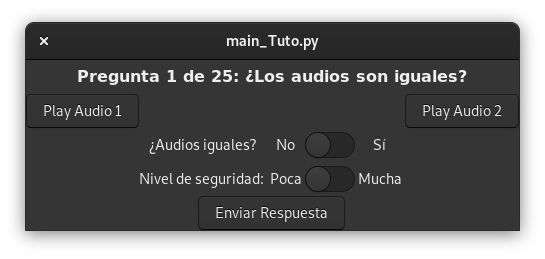
\includegraphics[scale=0.6]{../imagenes/interFin.png}
			        \centering
			        \caption{Apariencia de la interfaz del test.}
			        \label{fig:interfazTestFin}
                \end{figure}
                
                Todos los resultados se almacenan durante la ejecución del experimento en un archivo con terminación ``.csv'', que es el que se utiliza posteriormente para el análisis de los datos.
                
                Para la realización del test participaron un total de 31 personas con edades comprendidas entre los 19 y los 60 años. En la figura \ref{fig:participantes} se puede observar una imagen de varias de las mismas durante el transcurso del test.
                
                \begin{figure}
                    \includegraphics[scale=0.45]{../imagenes/participantes.png}
			        \centering
			        \caption{Varios de los participantes durante el transcurso de los tests.}
			        \label{fig:participantes}
                \end{figure}
            
            

\end{document}